
\chapter{Fundamentação teórica} \label{processamentoimagens}

\section{Processamento de imagens e Visão Computacional}

    A visão humana é considerada por muitos um sentido complexo e muito poderoso. Além disso, as imagens podem ser a parte mais importante da nossa percepção.  É natural então imaginar que cientista queiram reproduzir as características e capacidades da visão através de programas de computador. Mas enxergar, ou ver, é muito mais do que detectar obejtos em um ambiente. Envolve também analisar e encontrar características importantes e derivar informação do que foi percebido.\cite{graciano2007rastreamento} Reproduzir esse processo é uma tarefa de extrema dificuldade e com esse intuito surgiu a área de Processamento de imagens.

    O Processamento de imagens é uma disciplina que vem do processamento de sinais. Afinal de contas, uma imagem não passa de um conjunto de sinais luminosos detectados por um sistema de visão. Podemos definir imagens como uma função \textit{f(x,y)} onde x e y são coordenadas espaciais e o valor de  \textit{f(x,y)} é a luminosidade, ou nível de cinza, da imagem naquele ponto. Quando esses valores são todos discretos, chamamos essa imagem de uma imagem digital.\cite{gonzalez2009digital} Cada elemento individual dessa imagem, cada valor em cada coordenada, pode ser chamado de um \textit{picture element} ou mais comumente \textit{pixel}.

    O interesse em Processamento de imagens normalmente se aplica em duas grandes áreas. Aprimoramento e correção de imagens para fins de interpretação humana e algoritmos para análise automática de informações contidas em imagens. Alguns autores chamam a primeira área de Processamento de imagens e a segunda de visão computacional. Essa distinção é restritiva, pois implica de certa forma que um programa na área de Processamento de imagens deve ter uma imagem como entrada e saída, mas nesse caso, nem uma tarefa simples como encontrar a cor predominante em uma imagem estão

    Diferente dos humanos, softwares de processamento de imagem ou visão computacional, são capazes de extrair informações de imagens em espectros de frequência diferente, como o raio-x ou raios gamma. Computadores podem processar imagens de fontes que os olhos humanos não estão acostumados a processar.

    Um sistema de Processamento de imagens normalmente possui dois componentes crucias: o equipamento para aquisição da imagem e o \textit{software} de processamento propriamente dito. É importante lembrar que a aquisição da imagem não vem apenas de câmeras fotográficas ou de vídeo. Qualquer dispositivo físico sensível a alguma faixa do espectro eletromagnético capaz de adquirir um sinal nessa faixa e digitalizá-lo pode servir para adquirir a imagem. O processamento normalmente é determinado por algoritmos e formulações matemáticos e estatísticas. Porém intuição humana ainda é de grande importância na escolha das técnicas a serem utilizadas.

    O Processamento de imagens começou a ser aplicado na área de Jornalismo, na busca de aprimorar as imagens transmitidas por cabos submarinos entre Londres e Nova York. \cite{marques1999processamento} O grande salto na área, porém, ocorreu com o advento dos primeiro computadores digitais, trinta anos depois. Com o aumento das pesquisas inúmeras novas técnicas foram criadas nos laboratórios de computação da época.

    Desde então, o Processamento de imagens e a visão computacional tem sido usados em diversas áreas. De fato, quase não existe uma área de implementação tecnológica que não tenha sido impactada pelo avanço no Processamento de imagens. Na medicina, imagens são rotineiramente utilizadas para elaborar diagnósticos e é possível utilizar programas de computador para encontrar anomalias em imagens obtidas por máquinas como o raio-x. É possível contar células em uma imagem de microscópio ou galáxias em uma imagem de um telescópio espacial. Sistemas de identificação biométrica por impressão digital ou reconhecimento de retina são cada vez mais abrangentes pelo mundo. Técnicas de transmissão de sinal de imagem e compressão de vídeo possibilitam alguns dos serviços digitais mais utilizados atualmente. E finalmente, programas de visão computacional são capazes de detectar posição de veículos em um estacionamento.

    Nas seções seguintes deste trabalho, descreverei alguns conceitos e técnicas de Processamento de imagens importantes para a compreensão do funcionamento do programa proposto.

    \section{Histogramas} \label{histograma}
        O histograma de uma imagem com níveis de cinza entre 0 e 255 é uma função discreta $h(nc) = N$. Onde nc é um determinado nível de cinza e N é o número de \textit{pixels} na imagem que possuem esse nível.\cite{gonzalez2009digital} O histograma nada mais é que a representação gráfica da frequência da distribuição dos níveis de uma imagem.\cite{IBGE2000introducao}. Ele portanto informa a probabilidade de que um determinado pixel possua um certo nível de cinza. A imagem \ref{HistogramaFig} mostra uma imagem e um gráfico de barras que representa seu histograma.

        Histogramas também podem ser extraídas de imagens coloridas. Nesse caso, normalmente cada canal RGB é separado e um histograma para cada um desses canais é gerado. É comum que programas que usam o histograma de uma imagem dividam os valores encontrados em cada nível pelo número total  de \textit{pixels}, obtendo assim um histograma normalizado.

        A extração de histogramas é a base para diversas operações de processamento de imagem. Além de prover estatísticas importantes sobre a imagem, os cálculos de histogramas são pouco exigentes tanto para o \textit{software} quando para o \textit{hardware} e portanto são muito importantes para processamento em tempo real de vídeo.

        Alguns conceitos de qualidade de imagem, como constraste e brilho estão associados a histogramas. A forma do histograma sozinha pode servir para se determinar vários aspectos da imagem. O constraste de uma imagem é diretamente proporcional dos níveis de cinza da imagem, ou seja, é proporcional a largura do gráfico do histograma. O brilho por outro lado pode ser indicado pela média dos valores do histograma ou pelos picos mais a direita ou mais a esquerda do histograma, representando respectivamente brilho mais alto ou mais baixo.

        Uma utilidade comum do histograma são as chamadas técnicas de transformação de histograma. Nessas técnicas, uma função de transformação é aplicada sobre a função h(nc) do histograma a fim de deslocar os valores para níveis mais desejados. Uma função de transformação que torne a curva do histograma mais uniforme aumenta o contraste da imagem, enquanto outras podem aumentar a probabilidade de um determinado valor que se deseja dar destaque.

        Além disso, os histogramas podem ser utilizados para auxiliar em técnicas de segmentação, como será discutido na seção \ref{segmentacao}. A análise de um histograma pode ser crucial para a determinação de um limiar adequado para binarização. Na seção \ref{segmentacaoVeiculos} eu descrevo como o histograma de cada quadro do vídeo é utilizado para separar os veículos em movimento na imagem dos outros elementos estáticos.

\begin{figure}
 \centering
\begin{subfigure}{.5\textwidth}
  \centering
  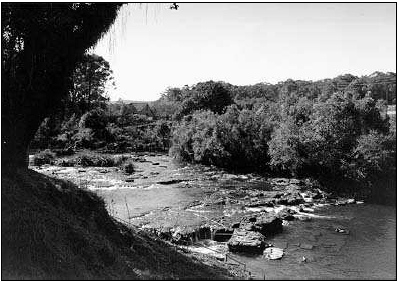
\includegraphics[width=.8\linewidth]{Imagem}
  \caption{}
  \label{histograma:sfig1}
\end{subfigure}\


\begin{subfigure}{.5\textwidth}
  \centering
  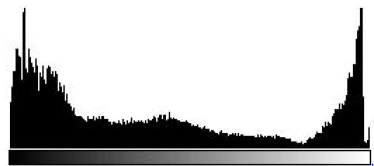
\includegraphics[width=.8\linewidth]{Histograma2}
  \caption{}
  \label{histograma:sfig2}
\end{subfigure}
\caption{(a) Uma imagem; (b)O seu histograma \cite{marques1999processamento}}
\label{HistogramaFig}
\end{figure}

    \subsection{Comparação de histogramas} \label{comparacaoHistogramas}

        Para algumas aplicações, é importante fazer comparações entre dois ou mais histogramas. Essas comparações podem revelar semelhanças ou diferença relevantes para imagens. Por exemplo, no caso desse trabalho, determinar se uma determinada região é mais semelhante a uma vaga vazia ou a um veículo qualquer. É possível também fazer essa operação para determinar eficiência de filtros ou de técnicas de normalização de histogramas.

        A comparação de histogramas consiste efetivamente em comparar duas amostras de distribuição de probabilidade. Sendo assim, várias técnicas utilizadas na área da Estatística são comumente aplicadas no Processamento de Imagens e Visão computacional. É comum se utilizar de métodos que calculam distâncias entre os diversos \textit{bins} ou seções do histograma. Um \textit{bin} é um separador que contém um intervalo dos dados que podem aparecer no histograma. Por exemplo, um histograma de uma imagem que contém 256 níveis de cinza pode possuir 256 \textit{bins} que representam um único nível de cinza cada um ou 25 \textit{bins} que representam a distribuição de um intervalo de 10 níveis de cinza cada. Comparações \textit{bin} a \textit{bin} assumem que os histogramas estão no mesmo domínio, o que normalmente não é um problema na área do Processamento de Imagens. Elas também dependem do número de \textit{bins} existentes. Se o número for pequeno, a medida da distância será robusta, mas pouco discriminativa, se for muito grande, a distância é discriminativa, mas não robusta.\cite{pele2010quadratic}

        Técnicas chamadas \textit{cross-bin}, que levam em conta diferenças além daquelas \textit{bin} a \textit{bin} existem e são bastante utilizada. Algumas delas são brevemente apresentadas em \cite{zhang2014comparison} e em \cite{rubner2000earth}. Em \cite{rubner2000earth} a técnica chamada de Distância do Movedor da Terra (\textit{Earth Mover's Distance}), derivada de comparação de grafos bipartidos e que consiste em avaliar o custo de se deslocar uma amostra - ou um histograma  - para que ela corresponda com a outra.

        Por conta das tecnologias utilizadas nesse trabalho e da natureza de sua implementação, técnicas de comparação \textit{bin} a \textit{bin} são mais interessantes do que as técnicas \textit{cross-bin}. Em particular, duas técnicas são de grande interesse para esse trabalho: a distância Qui-Quadrado e a técnica de comparação por intersecção.

        A técnica Qui-Quadrado ($\chi^{2}$) vem da área de comparação de distribuições probabilísticas onde é utilizada para testar semlhanças entre uma distribuição e as frequências observadas\cite{pele2010quadratic}.Ela dá mais importância às diferenças entre as \textit{bins} maiores do que entre as menores. Essa técnica é bastante utilizada para a classificação de objetos em imagens e identificação de imagens muito semelhantes. Ela é descrita pela fórmula:

        \begin{equation}\label{quiQuadrado}
          d(H_{1}, H_{2}) = \sum_{I = 0}^{N}\frac{(H_{1}(I) - H_{2}(I))^2}{H_{1}(I)}
        \end{equation}


        Onde $d(H_{1}, H_{2})$ é a diferença entre os dois histogramas $H_{1}$ e $H_{2}$ e $N$ é o número de \textit{bins} nos dois histogramas. Como é uma técnica de comparação entre \textit{bins}, $N$ deve ser o mesmo para os dois histogramas.

        A técnica da intersecção calcula a porção comum de dois histogramas e é particularmente útil em casos como: comparação de um mesmo objeto em ângulos de visualização diferentes, imagens com resoluções diferentes e verificação de diferenças no fundo das imagens que contém objetos. Nesse trabalho, essa técnica é utilizada para ajudar a determinar o estado das vagas no estacionamento. Esse processo é descrito na seção \ref{identificacaoFundo}.

        A diferença por intersecção pode ser descrita matematicamente como:

        \begin{equation}\label{intersecção}
          d(H_{1}, H_{2}) = \sum_{I = 0}^{N}min(H_{1}(I), H_{2}(I)
        \end{equation}

        Aonde, novamente, $d(H_{1}, H_{2})$ é a diferença entre os histogramas e $N$ é o número de \textit{bins}.


        Uma diferença importante entre as duas técnicas é que na comparação $\chi^{2}$, quanto menor o valor, mais semelhantes são os histogramas. No caso da intersecção, quanto maior o valor de $d(H_{1}, H_{2})$, maior a semelhança.

        \subsection{Equalização de histogramas} \label{equalizacaoHistogramas}

        Equalização ou normalização de histogramas é a técnica que procura redistribuir os valores percentuais de cada nível de cinza no histograma de uma determinada imagem. O objetivo é obter um histograma uniforme aonde a probabilidade de ocorrência de cada nível possível é praticamente a mesma. Utiliza-se para tal uma função de transformação aplicada sobre o histograma da imagem. A função mais comum utilizada para essa tarefa é a função de probabilidade acumulada dada por:

        \begin{equation}\label{intersecção}
          s_{k} = P(r_{k}) = \sum_{j = 0}^{k}p_{r}(r_{j})
          \caption{A equação $csf$ \cite{marques1999processamento}}
        \end{equation}

        Onde $P(r_{k})$ é o valor do nível $k$ de cinza no histograma e $p_{r}$ é a probabilidade de ocorrência deste nível na imagem e $s_{k}$ é o valor da saída.

        Aplicar técnica de equalização de histogramas é útil em diversas situações. Quando o processo é aplicado sobre uma imagem com predominância de níveis de cinza altos, tendendo ao branco, os valores se espalham por todo o espectro possível, melhorando o contraste da imagem e trazendo a tona detalhes que previamente podiam ser difíceis de se perceber.

        Quando o histograma de uma imagem escura, com valores tendendo a níveis baixos de cinza, os objetos escuros ficam mais claros e os claros ficam mais claros ainda. Apesar do aumento de claridade poder trazer perda de detalhes em seções mais claras, ele pode revelar e ajudar a detectar objetos que antes estavam escondidos em regiões muito escuras da imagem. No geral, a equalização de histogrmas tem um poder muito grande de aumentar o contraste em imagens. A figura \ref{equalizacaoHistogramasFig} demonstra esse poder de forma bastante convincente.

        Por causa disso, a equalizaçao é utilizada extensivamente em diversas áreas do Processamento de Imagens. Na medicina, pode ajudar médicos a fazerem diagnósticos melhores ao analisarem imagens médicas. Realçar fotos antigas que perderam o contraste também é uma tarefa que pode ser cumprida com essa técnica.

        É possível também executar a equalização do histograma de apenas uma parte da imagem. Isso serve no geral para realçar detalhes da imagem que podem ser mais interessantes que a imagem como um todo. Nesse trabalho, o histograma de trechos da imagem aonde se sabe que existe uma vaga de um estacionamento e se desconfia que um veículo estacionou é equalizado e comparado com um histograma de controle, como detalhado na seção \ref{identificacaoFundo}. Essa equalização, porém, é feita no histograma da imagem no espaço HSV de imagens e tem a função principal de preparar estes histogramas para as técnicas de comparação descritas na seção \ref{comparacaoHistogramas}.


        \begin{figure}
      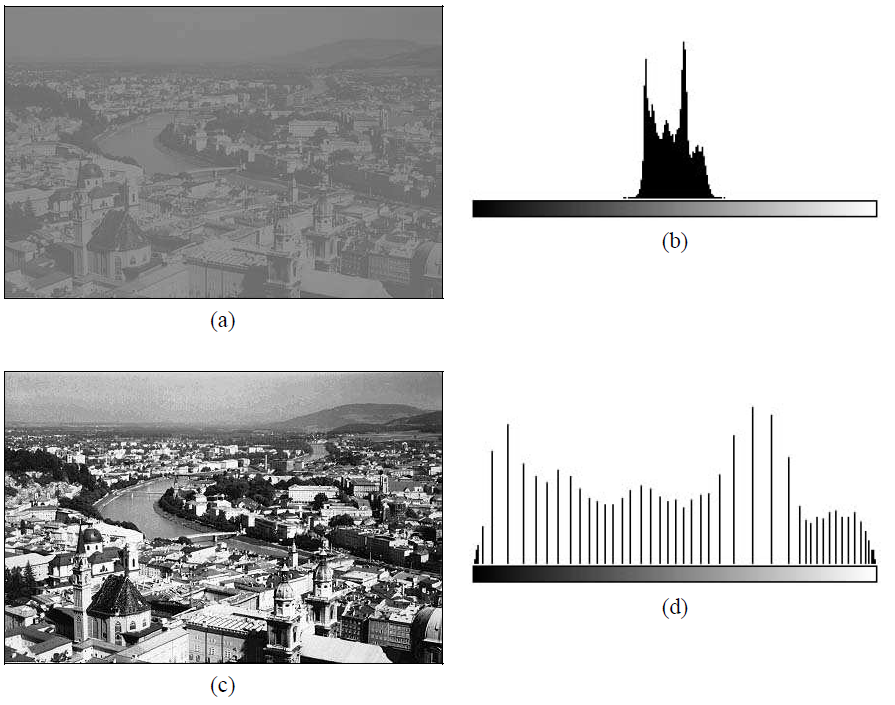
\includegraphics[width=1\textwidth]{equalizacaoHistograma}
      \caption{Aplicação da equalização de histograma a uma figura de baixo contraste. (b) mostra o histograma de (a) e (d) mostra o histograma de (c) \cite{marques1999processamento}}\label{equalizacaoHistogramasFig}
    \end{figure}










    \section{Segmentação de objetos} \label{segmentacao}
        Um processo importante para vários sistemas de visão computacional é o da extração de características ou \textit{features} importantes de uma ou mais imagens. Através destes \textit{features}o computador deve ser capaz de extrair uma informação ou conhecimento desejado, ou até mesmo mostrar na saída uma imagem diferente que possa ser analisada por humanos a fim de determinar essa informação.

        Quando o objetivo do processo é de localizar e extrair a posição de objetos específicos em uma cena, chamamos esse processo de segmentação de objetos. Ele consiste basicamente em isolar e selecionar \textit{pixels} da imagem de entrada que possam fazer parte da representação visual do objeto\cite{graciano2007rastreamento}. A saída desses programas pode ser uma imagem que contem apenas os objetos desejados, ou um arquivo com informações como o número de objetos encontrados diferentes encontrados.

        Existem diversas técnicas para segmentação de objetos descritas na literatura. Cada uma dessas técnicas é ideal para um tipo diferente de imagem ou de objeto a se encontrar. Assim como em muitas áreas da computação, a decisão da técnica a ser utilizada é tão importante quando a implementação do programa propriamente dito.

        É interessante apresentar alguns conceitos importantes antes de iniciar uma discussão sobre técnicas de segmentação. O primeiro deles é o conceito de vizinhaça do \textit{pixel}. A vizinhança de um ponto de uma imagem é um objeto de estudo importante para determinar objetos. Ela consiste essencialmente dos valores dos \textit{pixels} ao redor do \textit{pixel} sendo analisado. Chamamos de vizinhança-4 o conjunto dos quatro \textit{pixels} que ficam diretamente acima, abaixo, à direita e à esquerda do ponto em questão. A vizinhança-8, por sua vez, é então o conjunto que consiste da vizinhança-4 e mais os quatro \textit{pixels} nas diagonais do ponto sendo analisado. Chamamos os \textit{pixels} que fazem parte de alguma vizinhança de outro \textit{pixel} de vizinho.

        O segundo conceito importante é a definição de bordas. As bordas em uma imagem representam os limites de cada objeto e são, portanto, de extrema importância na segmentação de objetos em imagens. Pontos pertencentes a bordas são aqueles que possuem uma mudança brusca nos níveis de cinza. Por exemplo, podemos definir um ponto de uma borda em uma imagem binária - que possui apenas pontos brancos ou pretos - como um ponto preto que contenha pelo menos um vizinho branco.\cite{vkl1989jain}

        Uma técnica simples e muito utilizada para segmentação é da limiarização, ou \textit{thresholding}. Essa técnica consiste na categorização dos \textit{pixels} de uma imagem através de um limiar \textit{L}. Aqueles que possuirem valores maiores que \textit{L} terão seu valor configurado como o valor máximo, representado pela cor branca. Normalmente o valor do limiar é escolhido de acordo com a expectativa dos valores de cinza dos obejtos do conjunto de interesse da imagem, mas é possível também implementar formas de detectar um limiar apropriado computacionalmente. Na seção \ref{segmentacaoVeiculos} é descrito como o histograma de cada quadro foi usado para determinar um limiar global para a execução do \textit{thresholding} de cada \textit{frame}. O resultado é visível na figura \ref{LimiarizacaoFig}. É possível também, e apropriado em vários casos, determinar limiares locais para a imagem. Nesse caso, cada fragmento da imagem, como um quadrante, possui um valor diferente de \textit{L}. O resultado desse processo de limiarização é normalmente uma imagem binária.


\begin{figure}
 \centering
\begin{subfigure}{.5\textwidth}
  \centering
  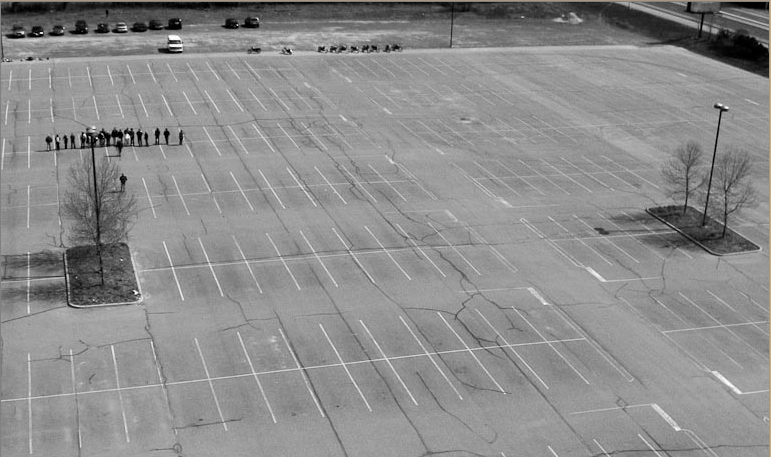
\includegraphics[width=.8\linewidth]{Estacionamento}
  \caption{}
  \label{Limiarizacao:sfig1}
\end{subfigure}\


\begin{subfigure}{.5\textwidth}
  \centering
  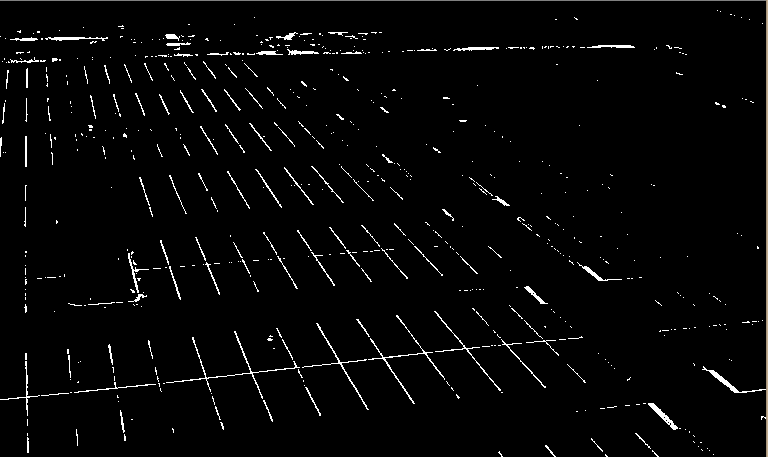
\includegraphics[width=.8\linewidth]{EstacionamentoBinarizado}
  \caption{}
  \label{Limiarizacao:sfig2}
\end{subfigure}
\caption{(a) Uma imagem de um estacionamento; (b) A mesma imagem binarizada através da técnica utilizada na seção \ref{segmentacaoVeiculos}}
\label{LimiarizacaoFig}
\end{figure}

    Uma vez que temos uma imagem binarizada podemos utilizar várias técnicas para separar os objetos. A mais simples de todas, nos casos onde a imagem contém apenas um objeto de interesse que possui valores brancos na imagem, podemos simplesmente encontrar todos os \textit{pixels} brancos. Em imagens binárias que possuem mais de um objeto de interesse é preciso implementar uma maneira de se separar esses objetos. Existem técnicas que analisam a conectividade dos pontos a fim de extrair limites dos objetos.\cite{vkl1989jain} Outros algoritmos classificam pontos com o valor de interesse em classes diferentes. Pontos com o valor interessante não-classificados que sejam vizinhos de um ponto de uma classe passam a fazer parte daquela classe ou passam a integrar uma classe nova caso contrário. Ao final da execução, cada classe contém os \textit{pixels} de um objeto diferente.

    Outra técnica interessante de separação de objetos em imagens é o algoritmo chamado \textit{watershed}. \textit{Watersheding} é um algoritmo morfológico que permite a detecção de bordas em imagens em níveis de cinza. É uma técnica muito eficiente e que produz contornos bastante precisos. Esse algoritmo possue uma desvantagem particular em relação a outros algoritmos de segmentação de imagens. Por vezes, se mal utilizado a técnica de \textit{watersheding} pode segmentar demais a imagem, reconhecendo objetos não existentes. Existem então, diversas pesquisas para minimizar esse problema, como a apresentada em \cite{malpica1997applying}.

    O algoritmo de \textit{watershed} consiste em interpretar a imagem como um mapa topológico de uma região, onde os pontos mais escuros representam pontos mais baixos, ou "vales". Uma vez detectados esses vales, o algoritmo começa um processo de inundação do vale, daí o nome. Computacionalmente, esse processo de inundação consiste na atribuição de classes a pixels adjacentes ao vale que se propaga a cada iteração. Os pontos onde a água se encontraria - ou pontos que seriam atribuídos a duas classes - são os pontos de borda da imagem. Essa técnica é muito usada no ramo da Biologia, para a segmentação de células em imagens de microscópio.

    É importante também diferenciar objetos encontrados em uma imagem um do outro. Muitas vezes a imagem binária resultante de um processo de segmentação contém diversos objetos. Em alguns casos, não temos interesse em todos eles e é importante que o computador seja capaz de diferenciar um do outro. Existem diversas técnicas que visam esse objetivo. É possível analisar o histograma apenas da região onde o programa sabe que existe um objeto e comparar com um histograma esperado. Outros algoritmos se utilizam de operações matricias que se aproximam de uma derivação a fim de encontrar a orientação das bordas do objeto do objeto detectado.

    Outra abordagem bastante utilizada é a de redes neurais treinadas para identificar esses \textit{features} de objetos de interesse. Objetos encontrados são analisados por uma técnica qualquer e suas características são encontradas. As redes são então treinadas para classificar objetos com as mesmas características junto com os seus semelhantes. Esse tipo de implementação já foi utilizada com sucesso em aplicações para gerenciamento de estacionamento, como a apresentada em \cite{true2007vacant}.

    Para a implementação programa apresentado nesse trabalho são de particular interesse as técnicas de segmentação baseadas em \textit{thresholding} e subtração de fundo. As técnicas de geração e subtração de fundo serão descritas mais adiante na seção \ref{background}. Além delas, as técnicas de reconhecimento de \textit{features} de objetos através de comparação de histogramas serão bastante utilizadas para a confirmação de que o objeto encontrado é um veículo.

    \section{Subtração de imagens}  \label{subtracao}

    A diferença entre duas imagens pode ser obtida através de uma subtração simples dos valores dos elementos da primeira imagem com os elementos correspondentes da segunda imagem. Matematicamente podemos expressar essa operação pela equação:
    \begin{equation}
        D(x,y) = A(x,y) - B(x,y)
    \end{equation}

    Onde $D(x,y)$, $A(x,y)$ e $B(x,y)$ são os valores dos \textit{pixels} na posição (x,y) das imagens de diferença obtida e as imagens A e B originais. Podemos subtrair imagens RGB fazendo a subtração normal de cada canal da primeira imagem com o canal correspondente da segunda.

    A grande utilidade de se subtrair duas imagens é justamente realçar as diferenças entre estas duas imagens. Obter a diferença de duas imagens pode ser útil para facilitar a visualização de resultados da aplicação de uma algoritmo ou para encontrar mudanças que ocorrem entre dois quadros distintos de um vídeo capturado. A diferença entre dois quadros de um vídeo contém a posição de um objeto que se moveu na cena, mais o ruído da imagem. Essa segunda aplicação mencionada é de grande relevância para este trabalho. Na seção \ref{segmentacaoVeiculos} mais a frente, eu descrevo como utilizei a diferença entre dois quadro consecutivos para encontrar uma região que contenha um veículo em movimento, e na seção \ref{geracaoFundo} mostro como utilizei essa região para separar dinamicamente o \textit{background} da imagem dos elementos de \textit{foreground}. Além disso, no algoritmo descrito na seção \ref{diferencasFundos} utilizo a diferença entre o fundo da imagem em dois momentos diferentes para detectar veículos que estacionaram nesse período de tempo e passaram a fazer parte do fundo.

    Se uma imagem composta por valores de níveis de cinza tem o valor de cada um dos seus \textit{pixels} representado por 8 bits, os valores que podem ser representados estarão então entre o intervalo de 0-255. Mas imagens resultantes da subtração de outras duas imagens terão seus valores representados na faixa de -255 a 255. É preciso então processar esses valores para trazê-los de volta para o intervalo que podemos representar. Existem diversas soluções para esse problema. Os algoritmos deste trabalho, porém, se importam apenas com a existência de uma diferença entre duas imagens e a posição dos \textit{pixels} que possuem valor maior que zero na imagem de diferença e não os valores específicos de cada um. Sendo assim, a abordagem utilizada para resolver essa situação foi apenas a extração do valor absoluto do resultado da diferença.

    A figura \ref{SubtracaoFig} ilustra a subtração de duas imagens. O resultado apresentado já passou por um processo de limiarização e portanto é uma imagem binária. As imagens utilizadas são fundos gerados dinamicamente. A imagem obtida pela subtração mostra uma diferença em uma região onde é sabido que há vagas no estacionamento. Na seção \ref{diferencasFundos} é descrito como essa informação é utilizada para determinar que um carro estacionou em uma vaga.

    %Colocar uma imagem de subtração de imagens%


    \begin{figure}
 \centering
\begin{subfigure}{.5\textwidth}
  \centering
  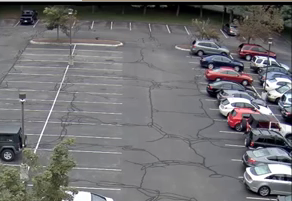
\includegraphics[width=.5\linewidth]{FigSubtracao1}
  \caption{}
  \label{Subtracao:sfig1}
\end{subfigure}%
\begin{subfigure}{.5\textwidth}
  \centering
  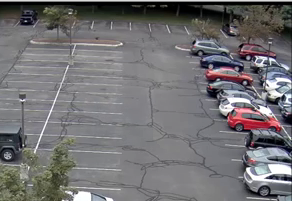
\includegraphics[width=.5\linewidth]{FigSubtracao2}
  \caption{}
  \label{Subtracao:sfig2}
\end{subfigure}


\begin{subfigure}{.5\textwidth}
  \centering
  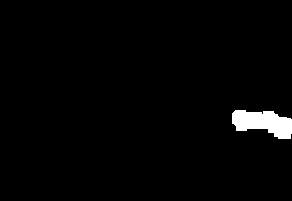
\includegraphics[width=.8\linewidth]{FigSubtracao3}
  \caption{}
  \label{Subtracao:sfig3}
\end{subfigure}
\caption{(a) O fundo em um determinado quadro em um vídeo; (b) O fundo em um outro quadro do mesmo vídeo alguns segundos depois; (c) A imagem resultante da subtração entre (a) e (b) binarizada.}
\label{SubtracaoFig}
\end{figure}



    \section{Operações Morfológicas} \label{morfologicas}
    O principio básico da morfologia matemática consiste em extrair as informações relativas à geometria e à topologia de um conjunto desconhecido (uma imagem), pela transformação através de outro conjunto completamente definido, chamado elemento estruturante.\cite{marques1999processamento} Para aplicar operações morfológicas então, precisamos primeiramente definir conjuntos sobre as imagens. Normalmente aplicamos as operações descritas a seguir em imagens binárias e essas imagens podem ser descritas completamente pelo conjunto A definido por:

    \begin{equation}\label{conjuntoA}
      A = {(x,y)|P(x,y) > 0}
    \end{equation}

    Ou, mais simplesmente, o conjunto dos \textit{pixels} $P(x,y)$ que não são pretos.

    O elemento estrutrante $B$ para as operações morfológicas é uma segunda matriz, de tamanho geralmente menos do que o da imagem original que deve ser escolhida cuidadosamente para que se obtenha os resultados desejados.

    As duas operações morfológicas básicas para o Processamento de imagens são: a dilatação, que aumenta os elementos de uma imagem alterando a área ao redor de um determinado \textit{pixel} para conformar a um dado padrão e a erosão, que se utiliza do elemento estruturante para remover objetos indesejados e diminuir elementos.\cite{de2006introduccao}.

    A dilatação faz com que um objeto presente na imagem cresça de tamanho. Ela é utilizada também para elminiar buracos em componentes segmentados, pois falhas menores do que o elemento estruturante B são completamente cobertas ao final da operação. Se chamarmos o conjunto de todos os pontos da imagem de $I$, podemos definir o conjunto resultante da operação de dilatação como:


    \begin{equation}\label{conjuntoDilatacao}
      D(A,B) = A \oplus B = \{{(x,y) \in I | B_{(x,y)} \cap A \neq \emptyset}\}
    \end{equation}

    Isto é, todos os elementos de $I$ aonde $B$, se deslocado para a posição (x,y) do elemento, intercepta o conjunto dos pontos brancos, $A$. A figura \ref{DilatacaoFig} ilustra o resultado do processo de dilatação.

    \begin{figure}
 \centering
\begin{subfigure}{.5\textwidth}
  \centering
  
\includegraphics[width=.4\linewidth]{ADilatar}
  \caption{}
  \label{Dilatacao:sfig1}
\end{subfigure}%
\begin{subfigure}{.5\textwidth}
  \centering
  
\includegraphics[width=.2\linewidth]{Elementoestruturante}
  \caption{}
  \label{Dilatacao:sfig2}
\end{subfigure}


\begin{subfigure}{.5\textwidth}
  \centering
  
\includegraphics[width=.4\linewidth]{Dilatada}
  \caption{}
  \label{Dilatacao:sfig3}
\end{subfigure}
\caption{(a) Uma imagem binária; (b) O elemento estrutrante a ser utilizada na dilatação; (c) A imagem resultando do processo de dilatação, com os pixels adicionados pintados de azul para facilitar a visualização}
\label{DilatacaoFig}
\end{figure}


    Nesse trabalho, a dilatação é utilizada na seção \ref{segmentacaoVeiculos} para aumentar a área da mancha encontrada pela diferença dos quadros consecutivos, a fim de determinar uma maior área que certamente pertence ao \textit{foreground}.

    A erosão por sua vez faz o processo contrário da erosão. Ela dimunui o contorno dos objetos, pode diminuir o número de componentes segmentados e até remover elementos que sejam menores do que o elemento estruturante, uma vez que componentes que sejam menores serão eliminados da imagem $I$. Uma aplicação interessante da operação de erosão é na detecção de contornos. Podemos subtrair uma imagem de sua versão erodida para encontrar os contornos dos objetos presentes na imagem.

    Da mesma forma que com a dilatação, podemos definir a erosão matematicamente como:

    \begin{equation}\label{conjuntoErosao}
      D(A,B) = A \ominus B = \{{(x,y) \in I | B_{(x,y)} \subseteq A}\}
    \end{equation}

    Ou seja, os pontos em $I$ tais que o elemento estruturante $B$ deslocado para a posição (x,y) do ponto, está contido completamente em A. Mais especificamente, apenas os pontos onde se sobrepusermos o $B$ só haverá pontos brancos sob os pontos de B. A figura \ref{ErosaoFig} ilustra o processo de erosão sobre uma imagem binária.

       \begin{figure}
 \centering
\begin{subfigure}{.5\textwidth}
  \centering
  
\includegraphics[width=.4\linewidth]{ADilatar}
  \caption{}
  \label{Erosao:sfig1}
\end{subfigure}%
\begin{subfigure}{.5\textwidth}
  \centering
  
\includegraphics[width=.2\linewidth]{Elementoestruturante}
  \caption{}
  \label{Erosao:sfig2}
\end{subfigure}


\begin{subfigure}{.5\textwidth}
  \centering
  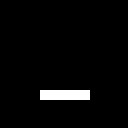
\includegraphics[width=.4\linewidth]{Erodida}
  \caption{}
  \label{Erosao:sfig3}
\end{subfigure}
\caption{(a) Uma imagem binária; (b) O elemento estrutrante a ser utilizada na erosão; (c) A imagem resultando do processo de erosão}
\label{ErosaoFig}
\end{figure}

    É possível também combinar essas operações entre si para criar novas operações morfológicas sobre as imagens. As combinações mais comuns formam as operações de abertura e fechamento. A abertura é a aplicação de uma dilatação seguida de uma erosão. A operação da abertura suaviza os contornos dos objetos na imagem, ou seja, ela remove pequenas protuberâncias. O fechamento por sua vez, é a combinação de uma erosão seguida de uma dilatação. Essa operação é utilizada para fechar pequenos buracos ou falhas contidos no interior de um objeto na imagem binária.


   \section{Geração de background} \label{background}

   Uma área de estudos de muita utilidade na segmentação de objetos é de geração de fundo. Em particular, segmentar os objetos que pertencem ao \textit{foreground} dos objetos que pertencem ao fundo da imagem é uma etapa crucial nos programas de segmentação ou rastreamento de objetos em vídeo. De fato, o primeiro passo nesses algoritmos normalmente é encontrar um fundo para servir de imagem de referência e possibilitar que sejam aplicadas técnicas de subtração de fundo com a finalidade de encontrar objetos que estejam em movimento.

   A abordagem típica de determinação de \textit{background} é obter a imagem de referência para o fundo quando a cena está estática.\cite{shoushtarian2003practical}. Na prática essa abordagem não é totalmente eficiente, principalmente em aplicações que dependem de imagens obtidas de câmeras de segurança ou de ambientes que não costumam ficar totalmente sem movimento. Em programas que obtém as imagens através de câmeras que filmam o mesmo ambiente durante um dia inteiro, mudanças na iluminação, tanto natural quanto artificial, modificam o fundo da imagem. Além disso, objetos que estavam em movimento podem se tornar objetos estáticos e devem ser agregados ao \textit{background}.

   É preciso então encontrar técnicas para determinar o fundo da imagem em tempo de execução, de forma adaptativa e dinâmica. Alguns programas se utilizam da média aritmética ou dos quadros durante o decorrer do vídeo. Similarmente a observar apenas uma imagem, pode-se observar a mediana dos valores de cada \textit{pixel} dos quadros. O algoritmo apresentado em \cite{shoushtarian2003practical} se utiliza de temporizadores para atualizar os valores dos pixels de fundo e em \cite{chen2012dynamic} é apresentado ainda um outro método.

   Esse trabalho se utiliza de uma técnica de geração de fundo similar àquela apresentada em \cite{hai2009self} que provou ter grande sucesso na determinação de imagens de fundo em câmeras de monitoramento de trânsito. O algortimo é descrito com mais detalhes na seção \ref{geracaoFundo}.



    \section{Espaços de cor} \label{espaçosCor}

    A percepção de cor não é nada mais do que uma reação gerada no sistema visual humano quando a luz estimula as células presentes na retina. Dentre essas células, as importantes para a representação e interpretação de imagens são os cones, dos quais existem três tipos. Essas células são responsáveis pela interpretação de cor no olho humano. Como existem exatamente três tipos diferentes de cones, podemos descrever uma cor com exatamente três componentes numéricos, desde que apropriadamente ponderados.\cite{plataniotis2000color}. Um modelo de representação de cores é chamado de um espaço de cor.

    Antes de apresentar os espaços de cor relevantes ao trabalho, é interessante definir alguns conceitos importantes:

    \begin{itemize}
       \item O brilho (Br) é o atributo que define a sensação visual de que uma determinada área de uma imagem emite mais ou menos luz.
       O brilho de uma imagem é parcialmente responsável pela seu valor de luminosidade (L).
       \item A matiz da cor(Hue ou H) é o valor associado ao comprimento de onda predominante de uma determinada cor. A visão humana se utiliza principalmente deste atributo para diferenciar e identificar cores. Quando falamos que um objeto é vermelho, verde ou amarelo, normalmente estamos falando da matiz da cor do objeto.
       \item A saturação (S) se refere a "pureza" da cor ou ao quanto a matiz da cor está intocada. Em termos formais, a saturação é inversamente proporcional a quantidade de luz branca misturada a matiz.
     \end{itemize}

     Existem diversos espaços de cor diferentes. Alguns baseados em especificações de dispositivos, outros que visam simular a percepção real de cores e alguns que procuram separar valores importantes na representação da imagem. Cada um deles tem uma aplicação distinta. Nesse trabalho dois espaços são mais relevantes: o espaço RGB e o espaço HSV.

     \subsection{O espaço RGB}\label{RGB}

     RGB é um acrônimo para \textit{Red, Green, Blue}, vermelho, verde e azul em inglês. Essas são cores primárias que quando adicionadas corretamente podem gerar qualquer outra cor. Nesse espaço, a cor de cada \textit{pixel} em uma imagem é representada por um vetor de três coordenadas onde cada uma representa a quantidade de uma das três cores presentes no \textit{pixel}. Sendo assim, ele é considerado um sistema aditivo.

     O espaço RGB é o mais conhecido e provavelmente mais popular dos espaços de cor. Ele é uma escolha muito comum para representação digital de imagens, já que a maioria dos dispositivos de saída de imagem se utilizam da adição do vermelho, verde e azul para gerar as cores desejadas em cada \textit{pixel}. Por causa disso, utilizar o formato RGB traz diversas vantagens no quesito de arquitetura e elaboração de um sistema.

     O espaço RGB pode ser interpretado como um cubo, aonde os três eixos correspondem ao valor de vermelho, verde e azul.  O vértice no canto inferior aonde o valor de cada cor é 0 representa o preto, e o vértice oposto a ele representa o branco.\cite{ford1998colour} A diagonal que liga esses dois vértices representa então diversos níveis de cinza.

     Esse espaço apresenta algumas desvantagens. Uma delas é que no geral ele é dependendte do dispositivo sendo utilizado. Isto é, monitores diferentes apresentam discrepâncias ao mostrar imagens que têm os mesmo valores RGB em cada pixel. Além disso, ele não é muito ideal para representação de imagens reais, como fotografias ou imagens impressas. Isso é porque para formar corretamente uma cor cada componente RGB deve estar dentro da mesma largura de banda. Mas o maior problema com o espaço RGB para processamento de imagens é que ele traz algumas dificuldades para o processamento. Por exemplo, se um programa quer modificar a cor de uma determinado parte de uma imagem ou aumentar a intensidade luminosa de um \textit{pixel}, todos os três valores RGB devem ser recuperados e modificados apropriadamente um a um e depois atualizados. Sendo assim, para muitas aplicações em visão computacional, uma transformação do espaço RGB, chamada HSV, descrita na subseção \label{HSV} é utilizada.

     \subsection{O espaço HSV}\label{HSV}

     O espaço de cores HSV (\textit{Hue, Saturarion, Value} ou Matiz, saturação e valor) é um espaço de cores feito para ser mais intuitivamente legível para humanos. Como definimos as cores principalmente através dos valor de matiz e saturação, esse espaço se aproveita disso para representar cores de uma forma que seja mais fácil e intuitivo de se escolher uma cor do que no RGB. O atributo \textit{value} se refere a uma medida de luminosidade do ponto.

     Esse espaço não é nada mais da que uma deformação do cubo RGB e pode-se transformar facilmente uma imagem entre um formato e outro. De fato, os algoritmos são simples e todas as bibliotecas especializadas fornecem funções próprias para essa transformação. Ele é representado através de um círculo ao redor da linha diagonal que liga os vértices que representam o preto e o branco no cubo RGB. A posição do círculo nessa reta indica a luminosidade do ponto, enquanto a matiz é representada por um ângulo no círculo e a saturação pela distância radial do eixo de luminosidade para a cor. A figura \ref{figConeHSV} mostra uma representação visual destes conceitos.
     
     \begin{figure}
     \centering
      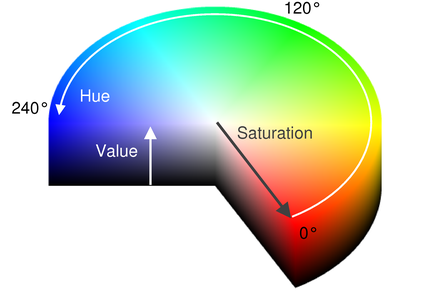
\includegraphics[width=.5\textwidth]{hsv}
      \caption{Representação visual do funcionamento do espaço de cor HSV}\label{figConeHSV}
    \end{figure}

     
     Tratar imagens no espaço HSV traz várias facilidades. É possível mudar os atributos da imagem ou de uma pequena seção da imagem modificando apenas um valor. Por exemplo, se uma aplicação deseja modificar as cores de uma imagem, basta recuperar os valores da matiz de cada ponto de cor e modificá-lo em uma certa quantidade de graus. Porém, como ele não passa de uma transformação do espaço RGB, a maioria das desvantagens apresentadas na subseção \ref{RGB} continuam presentes.

     Porém, a importância desse espaço de cor no processamento de imagens não vêm da capacidade intuitiva de se escolher uma determinada cor. Ele é muito relevante porque separa as informações de cor e luminosidade em cada ponto da imagem. Essa separação é muito importante para diversas aplicações. Ao equalizar histogramas por exemplo, é recomendado que o processo seja aplicado sobre o canal de luminosidade da imagem. Isso evita que as cores da imagem sejam modificadas de forma exagerada. Outra situação relevante é a de sombras ou outras mudanças de iluminação em reconhecimento de objetos ou regiões conhecidas. Quando uma área ou objeto está sobre algum efeito de iluminação, normalmente a maior modificação é no componente de luminosidade do ponto, enquanto a matiz da cor continua inalterada. Isso permite o reconhecimento de objetos ou de semelhanças mesmo sobre condições de iluminação diferentes. Por isso esse trabalho se utiliza do componente H de trechos de imagens para a comparação de histogramas na seção \ref{testesEstaticas}.
     
     \section{Classificação de objetos} \label{classificacao}
     
     Classificação de objetos em imagens consiste no agrupamento de objetos que foram vistos pelo sistema em classes diferentes. Esse processo se assemelha bastante ao reconhecimento de objetos em imagens. De fato, pode-se argumentar que reconhecer objetos individualmente é uma forma de classificar objetos aonde cada objeto compõe uma classe diferente.
     
     Objetos podem ser classificados com relação a várias características como cor predominante, tamanho, forma e muitas outras. Normalmente se escolhe parâmetros que sejam independentes entre as classes e diferenciem suficientemente objetos de classes distintas. O processo em si normalmente é feito se utilizando de alguma forma de rede neural. Uma vez determinados os parâmetros a serem utilizados, um conjunto de treinamento é criado.
    
     Para criar o conjunto inicial de imagens de treinamento para a rede neural responsável pela classificação, assume-se que o desenvolvedor esteja munido de uma aplicação capaz de detectar os atributos relevantes nas imagens. Quando esse é o caso, esse programa é expostos a diversas imagens contidas nas diferentes classes que se deseja separar. Ele determina os atributos presentes na imagem e então um usuário atribui aquela imagem a uma das classes. O programa então armazena a distribuição de valores para cada atributo através das imagens.  O passo seguinte é determinar um ponto de separação de cada classe para cada um dos atributos. Uma vez que os valores de atributo associados a cada classe são determinados, o programa é exposto a um conjunto de testes. A partir das informações obtidas na etapa de treinamento, o programa é capaz de classificar os objetos em uma imagem com sucesso.
     
     Por exemplo, suponha que um desenvolvedor queira elaborar um sistema que diferencia laranjas de limões. Uma possível solução é o uso da classificação de objetos em imagens. Para isso, o desenvolvedor iria expor seu programa a centenas de imagens de laranjas e de limões. As imagens de laranja são predominantemente laranjas, enquanto as de limão são predominantemente verdes. Esses então são atributos ideiais para a classificação. Esse programa então iria elaborar uma distribuição dos valores de laranja e verde de cada imagem exibida a ele. Munido dessa distribuição, basta determinar um limiar que separe as duas cores suficientemente. Dessa forma, se o valor de uma dessas cores está acima dessa limiar, é muito provável que a imagem seja da fruta correspondente à cor. Assim, o programa é capaz de distinguir entre imagens de laranjas e limões.
     
     
    


    